\section{Siamese Multi-Object Tracking and Embedding}
\label{sec:SiamMOTandFeatureEmb}

% ##############################################################################
\subsection{Motivation}

One of our experiments involved an end-to-end training of the \gls{siammot} together with a custom head aimed at embeddings based on \gls{roi}-pooled features for the object \gls{bbox}. The goal was to force the training process into extracting features that are not only satisfactory for detection and tracking but also do contain the necessary information to create embeddings for \gls{reid} purposes during the inference. We strived for simplicity by extending the processing pipeline without altering the existing infrastructure.

During research related to our Siamese tracking survey~\cite{ondrasovic2021siamese}, we noticed one work where the exemplar features were projected using \gls{gap} into an embedding space consisting of fewer dimensions~\cite{li2020figsiam}. The embedding vector was produced using the feature tensor representing the kernel for the cross-correlation operation. More concretely, let the extracted features be represented by an $8 \times 8 \times 256$ tensor. Then, the \gls{gap} along the channel dimension would produce a $1 \times 1 \times 256$ tensor, which could then be further flattened into a single $256$D vector. In the end, the obtained vector was $l_2$-normalized and thus projected onto a unit hypersphere. In the work of Li~\etal{}~\cite{li2020figsiam}, these embedding vectors were exploited for template updating and for combining multiple templates within a pool of size $n$ in an exponential fashion.

This observation led us to the following hypothesis. Given the fact the Siamese exemplar features do contain some, although probably not sufficient information for pure object \gls{reid}, would it be possible to map them further using a non-linear function to produce embedding vectors that could serve for \gls{reid}? Such features are just a learned template, therefore, some notion of similarity needs to be already built into it.

% ##############################################################################
\subsection{Feature Embedding Head Architecture}

% ------------------------------------------------------------------------------
\begin{figure}[!t]
    \centering
    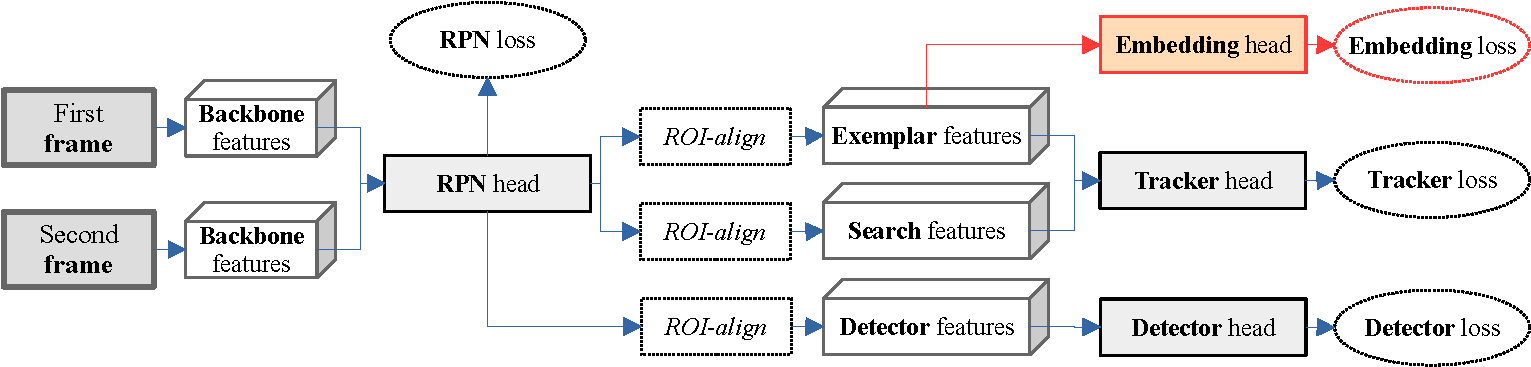
\includegraphics[width=\linewidth]{figures/siamese_tracking/siammot_feature_emb_training.pdf}
    \caption[Embedding-enhanced \gls{siammot} architecture]{Our extension (shown in red) to the underlying \gls{siammot} architecture that incorporates vector embeddings to the end-to-end training. This diagram shows the pipeline that is used during the training, not inference.}
    \label{fig:SiamMOTWithEmbeddings}
\end{figure}
% ------------------------------------------------------------------------------

As for the vector embedding computation, we attached an \gls{femb} head (\tabletext{}~\ref{tab:FeatureEmbeddingHead}) after the \gls{roi}-pooling phase of the backbone features (\figtext{}~\ref{fig:SiamMOTWithEmbeddings}). This ensured fixed tensor shapes and allowed us to process the very same features that the object detector and Siamese tracker utilized, too. Simply put, for every proposal made for a particular frame, we looked at the delineated \gls{bbox} through the lens of \gls{roi}-pooling to extract its features. We simply reused the extracted exemplar features. Later on, we processed these features using our newly devised \gls{femb} head to produce \gls{femb}. The resulting embeddings were subjected to the triplet loss computation with all the necessary operations such as various types of hard negative mining.

\begin{table}[!t]
    \centering
    \begin{tabular}{lll}
        \toprule
        \textbf{layer}    & \textbf{tensor shape}        & \textbf{parameters no.} \\
        \midrule
        input             & $\sbrackets{B, 128, 15, 15}$ & $0$                     \\
        \midrule
        conv $3 \times 3$ & $\sbrackets{B, 128, 13, 13}$ & $147\ 456$              \\
        ReLU              & $\sbrackets{B, 128, 13, 13}$ & $0$                     \\
        \midrule
        conv $3 \times 3$ & $\sbrackets{B, 256, 11, 11}$ & $294\ 912$              \\
        ReLU              & $\sbrackets{B, 256, 11, 11}$ & $0$                     \\
        \midrule
        flatten           & $\sbrackets{B, 30976}$       & $0$                     \\
        linear            & $\sbrackets{B, 1024}$        & $31\ 720\ 448$          \\
        \midrule
        $l_2$-normalize   & $\sbrackets{B, 1024}$        & $0$                     \\
        \bottomrule
                          & \textbf{total}               & $32\ 162\ 816$          \\
        \cline{2-3}
    \end{tabular}
    \caption[\gls{femb} head]{Our custom \gls{femb} head that we used to process backbone-extracted features to produce embedding vectors. It is built from two convolutional layers separated by a \gls{relu} nonlinearity followed by a fully connected layer that produces a $1024$ dimensional feature embedding. The batch size dimension is given by $B$ in the tensor shape. Since each embedding vector is normalized to unit length, we avoided learning biases throughout the whole network.}
    \label{tab:FeatureEmbeddingHead}
\end{table}

% ##############################################################################
\subsection{Training Phase}

The training phase was altered by adding another loss function to the sum of already existing three losses from the original model. In particular, the general \gls{siammot} loss function defined in \eqtext{}~\ref{eq:SiamMOTGeneralLoss} was reformulated as
\begin{equation}
    \label{eq:SiamMOTFeatureEmbLoss}
    \lossf = l_{rpn} + l_{detect} + l_{motion} + l_{emb}.
\end{equation}
The $l_{emb}$ loss incorporated a triplet loss (\eqtext{}~\ref{eq:TripletLoss},~p.~\pageref{eq:TripletLoss}). We also experimented with a contrastive loss (\eqtext{}~\ref{eq:ContrastiveLoss},~p.~\pageref{eq:ContrastiveLoss}), but the effect was detrimental in every aspect as expected, so we will not discuss it any further.

As we remarked in \sectiontext{}~\ref{sec:LatentSpacesAndEmbeddings},~p.~\pageref{sec:LatentSpacesAndEmbeddings}, aimed at latent spaces and embeddings, it is crucial to adopt appropriate sample mining strategies when using the triplet loss. The rationale is that for the training to keep progressing, the model needs to encounter harder and harder triplets to generate sufficient learning signals. To this end, we went for the semi-hard triplet mining strategy (\eqtext{}~\ref{eq:BatchHardMining},~p.~\pageref{eq:BatchHardMining}). However, we struggled with collapsing embeddings~\cite{levi2021rethinking}. This phenomenon happens when the embedding training forces the model to project all the features onto a single point in the embedding space, thus incurring the loss equal to the used margin. We claim that the use of semi-hard negative mining produced triplets that were too difficult. Since we used all the \gls{rpn} proposals to generate triplets, one may imagine that there would always be proposals covering only some small part of the object, making it problematic for the network to learn the concept of ``similarity'' and ``difference'' if it only processes very hard images. Nevertheless, these situations are very common in margin-based losses~\cite{levi2021rethinking}. The computed loss is so high that it is more suitable for the model to map all the features onto a single point. To remedy this, we implemented a batch-all online mining strategy (\eqtext{}~\ref{eq:BatchAllLossFunction},~p.~\pageref{eq:BatchAllLossFunction}), which stabilized the training.

We recommend first utilizing the batch-all mining strategy during the training, and then proceeding to a batch-hard strategy after a certain point. However, this approach would be time-consuming to find the right hyperparameters. There are many open questions, such as how to mine the \gls{rpn} proposals in a better way or how to set the margin value. Loss functions aimed at object \gls{reid} are notoriously cumbersome to train. We implemented the entire mining algorithm followed by the loss computation in a \gls{gpu}-only fashion for fast execution and easy integration into the pipeline.

% ##############################################################################
\subsection{Inference Phase}

\subsubsection{Feature-based Non-Maximum Suppression}
\label{sssec:FeatureNonMaximumSuppression}

Salscheider~\cite{salscheider2020featurenms} proposed an extended \gls{nms} algorithm that incorporates a distance between feature embeddings dubbed as \featurenms{} (\algtext{}~\ref{alg:FeatureNMS}). Considering our idea introduced above, we had to encompass the vector embeddings into the solver reasoning. In the beginning, we came up with a solution that exactly copied the one the mentioned author proposed. That provided further justification for attempting to implement the algorithm and test it in practice. The advantage is that this approach is restricted to the inference phase, thus experimenting with it does not require model re-training.

\def\threshlower{\tau_{\text{lower}}}
\def\threshupper{\tau_{\text{upper}}}
\def\threshsim{\delta}

We assume the reader is acquainted with the \gls{nms} algorithm (\sectiontext{}~\ref{ssec:NonMaximumSuppression},~p.~\pageref{ssec:NonMaximumSuppression}). Here we repeat the same definitions for clarity. Let $\mset{B} = \cbrackets{\vect{b}_1, \vect{b}_2, \dots, \vect{b}_n}$ be a set of $n$ region proposals described by $n$ \glspl{bbox}. Scores for each detection are contained in a set $\mset{S} = \cbrackets{s_1, s_2, \dots, s_n}$, where $s_i$ denotes a detection score for the $i$-th box, $\vect{b_i}$. This time, we are also going to need the associated feature embedding vectors with each \gls{bbox}, represented by a set $\mset{E} = \cbrackets{\vect{e}_1, \vect{e}_2, \dots, \vect{e}_n}$. Let $\mset{B}_{fnms}$ be  the set of filtered proposal instances from the set $\mset{B}$ produced by the \featurenms{} algorithm. The distinction in parameters is the following. The original algorithm requires only one threshold for the maximum allowed portion of the overlap between regions. The \featurenms{} requires three parameters discussed below.
\begin{itemize}
    \item A minimum threshold $\threshlower$ denoting a boundary below which the two objects are deemed as different. This value should be low, for example, $0.2$, which means that if the \gls{iou} between the two objects is less than $0.2$, then the two instances should be treated as different objects.
    \item A maximum threshold $\threshupper$ denoting a boundary above which the two objects are considered identical. Unlike the $\threshlower$, this value should be high, \egtext{}, $0.8$, indicating that if the \gls{iou} of the two object instances surpasses this threshold, then it should be the same object. The \gls{bbox} with the lower confidence is discarded.
    \item A threshold $\threshsim$ is used as a decision boundary between the embedding vectors. This threshold should reflect a measure of similarity. If the adopted measure of similarity falls below $\threshsim$, then the two objects are different, otherwise, they are considered the same. This value of $\threshsim$ is used only if the two conditions above do not hold.
\end{itemize}

\begin{algorithm}[t]
    \caption[\featurenms{} algorithm]{\featurenms{} algorithm.}
    \label{alg:FeatureNMS}
    \begin{algorithmic}[1]
        \Function{Feature-NMS}{$\mset{B}$, $\mset{S}$, $\mset{E}$, $\threshlower$, $\threshupper$, $\threshsim$}

        \State $\mset{B}_{fnms}$ $\gets$ $\emptyset$
        \Comment{initialize the output (filtered) set of region proposals}

        \While {$\mset{B} \neq \emptyset$}
        \Comment{loop until all the proposals are processed}

        \State $m \gets \underset{i \in \cbrackets{1, 2, \dots, \msetsize{S}}}{\argmax{}} \mset{S}$
        \Comment{find an index of a proposal with the highest score}

        \State $\mset{B} \gets \mset{B} - \vect{b}_m$, $\mset{S} \gets \mset{S} - s_m$, $\mset{E} \gets \mset{E} - \vect{e}_m$
        \Comment{remove the proposal}

        \State $\mset{B}_{fnms} \gets \mset{B}_{fnms} \cup \vect{b}_m$
        \Comment{save the proposal with the highest score}

        \For{$i \gets 1$ to $\msetsize{B}$}
        \Comment{iterate through remaining proposals}

        \If{\Call{iou}{$\vect{b}_m$, $\vect{b}_i$} $\geq \threshlower$}
        \Comment{above the lower-bound threshold}

        \If{\Call{iou}{$\vect{b}_m$, $\vect{b}_i$} $\geq \threshupper$}
        \Comment{above the upper-bound threshold}

        \State $\mset{B} \gets \mset{B} - \vect{b}_i$, $\mset{S} \gets \mset{S} - s_i$, $\mset{E} \gets \mset{E} - \vect{e}_i$
        \Comment{remove the proposal}

        \Else

        \If{\Call{similarity}{$\vect{e}_m$, $\vect{e}_i$} $\geq \threshsim$}
        \Comment{similarity above threshold}
        \State $\mset{B} \gets \mset{B} - \vect{b}_i$, $\mset{S} \gets \mset{S} - s_i$, $\mset{E} \gets \mset{E} - \vect{e}_i$
        \Comment{remove the proposal}
        \EndIf

        \EndIf
        \EndIf
        \EndFor
        \EndWhile

        \State \Return $\mset{B}_{fnms}$
        \EndFunction
    \end{algorithmic}
\end{algorithm}

% ##############################################################################
\subsection{Experimental Evaluation and Discussion}

The proposed embedding-based enhancement was evaluated against the baseline model without the \gls{femb} head. For a fair comparison, we made sure that the hyperparameters were identical to the greatest possible extent. We only had to alter the batch size and the learning rate. Since the triplet loss requires the computation of a large number of triplets, especially the batch-all strategy, we had to decrease the batch size and employ \gls{ga} to avoid crashes due to not having enough \gls{gpu} \gls{vram} available.

We can tell that this experiment was also detrimental to the tracker's performance. We conjecture that it was solely caused by the introduction of the \gls{femb} head itself. Our ablation study also demonstrated that joint training with the \gls{femb} head harmed the tracker, even if the original solver was adopted during the evaluation. This raises the question of potential task/feature conflict between the heads. We venture to claim there is an inherent incompatibility between the detection, tracking, and \gls{reid} tasks, despite the existence of a recently published work Lu~\etal{}~\cite{lu2020retinatrack}, who developed their \retinatrack{} tracker. Their framework exploited the base visual object detector called a \retinanet{}~\cite{lin2018focal} and then added, in principle, a very similar head as we did to produce embeddings. However, there are obvious architectural differences between the two trackers in terms of how the inference phase is executed.

\begin{table}[!t]
    \centering
    \begin{tabular}{llllll}
        \toprule
        \textbf{\gls{femb} head} & \textbf{solver} & \textbf{MOTA} & \textbf{MOTP} & \textbf{precision} & \textbf{recall} \\
        \midrule
                                 & original        & $0.7416$      & $0.1478$      & $0.9454$           & $0.7896$        \\
        \checkmark               & \featurenms{}   & $0.6861$      & $0.1568$      & $0.9166$           & $0.7574$        \\
        \checkmark               & original        & $0.6882$      & $0.1568$      & $0.9184$           & $0.7574$        \\
        \bottomrule
    \end{tabular}
    \caption[The effect of \gls{femb} head inclusion]{Demonstration that introduction of the \gls{femb} head causes a feature conflict on the level of backbone before the \gls{roi}-pooling operation. The effect is clearly visible since the \featurenms{} algorithm is only part of the inference phase. Both the object detection and the tracking head are ``parallel'' to the \gls{femb} head, however, training with the \gls{femb} head and then avoiding it during the inference considerably reduces the tracker's accuracy. The last two rows are practically identical in terms of \gls{clear} evaluation.}
    \label{tab:OrigSolverVsFeatureNMS}
\end{table}

To see the aforementioned feature conflict, one of the key takeaways from this trial, \tabletext{}~\ref{tab:OrigSolverVsFeatureNMS} shows that training the model with the \gls{femb} head and then evaluating it without the \featurenms{} algorithm, \ietext{}, using the original solver algorithm (\figtext{}~\ref{fig:SiamMOTOnlineSolver}), resulted in a drastically reduced tracker's accuracy. The reason is that the \gls{roi}-pooled features were trained in a conflicting way, therefore no task was served satisfactorily. Having trained the model and then omitting the \gls{femb} head completely during the testing should not dramatically affect ``parallel heads''. However, once the entire end-to-end model tries to accommodate for the triplet, object detection, and tracking loss functions, the conflicting nature of these tasks manifests itself in a negative fashion. This table shows the best models given by the combination of \gls{mota} and \gls{motp} metrics. All models were trained with \gls{ga} using batch size of $32 = 16 \times 2$ with $256$ object proposals. The relatively big batch size was dictated by the unstable nature of the triplet loss training.

Although this extension is not appropriate for practical usage unless further modifications are devised, we still wanted to evaluate the impact on inference speed in terms of \gls{fps} for comparison with the next experiment. It can be seen that the reduction in the tracker's speed is noticable. Specifically, the original model inference runs on average at $26.49$ \gls{fps}, whilst the \fembmodel{} version achieves $18.57$ \gls{fps}, resulting in reduction speed of about $30$\% (more in \tabletext{}~\ref{tab:InferenceSpeedComparison},~p.~\pageref{tab:InferenceSpeedComparison}).

\subsubsection{``Unfairness'' between the detection and re-identification}

There is a recent publication~\cite{zhang2021fairmot} by Zhang~\etal{} that discusses the notion of ``fairness'' between detection and \gls{reid}. According to their empirical evidence, there are multiple levels of ``unfairness''. This term was used to describe a situation in which the importance of either \gls{reid} or the detection task is lessened. We would like to emphasize the recency of this work (the end of $2021$) since several of their remarks and conclusions coincide with ours. Had this paper been published before conducting our experiments, we would have taken a different path, or at least we would have striven to find another way to incorporate the embeddings into an end-to-end pipeline. The aforementioned work, among other things, introduces a joint tracker that effectively circumvents the obstacles related to conflicting tasks. This framework avoids the use of anchor proposals and is based on \gls{centernet}~\cite{zhou2019centernet} object detector.

They argue that the \gls{reid} task may become overlooked if the embedding vectors are produced solely from the \gls{roi}-pooled regions, as in our case. Consequently, the detection task becomes central in terms of influence upon the loss function since generating embedding vectors on incorrect \glspl{bbox} is meaningless. Thus, the bias to produce accurate object proposals is inescapable.

Next, a problem arises when one anchor corresponds to multiple identities, which is an obstacle we have already mentioned (\sectiontext{}~\ref{ssec:SiamMOTAndReIDDiscussion}). As a result, the extracted features are not optimal in terms of their accuracy as well as discriminative representativeness. To remedy this, features should be extracted at a single point, \ietext{}, at the estimated object centers (hence the use of \gls{centernet}), instead of region proposals.

An analogical problem is when multiple anchors correspond to one identity. A high overlap in terms of \gls{iou} directs the model to estimate the same identity for nearby anchors. But, even a small perturbation may result in falling below a specific threshold and the anchors become marked as belonging to different objects. This situation is very common as proposals are generated on the feature level (a coarse representation due to downsampling), and not on the pixel level.

Another inherent problem when merging object detection and \gls{reid} is feature conflict. We have highlighted numerous times the significance of multi-layer feature fusion. However, not all tasks benefit from this approach equally. In particular, object detection utilizes high-level features to estimate object classes and locations, whereas the \gls{reid} is more prone to utilizing low-level features owing to their discriminative power. For that reason, it is important to balance the loss optimization.

Last but not least, the feature dimension poses another source of imbalance. The authors remarked that learning lower-dimensional features for the \gls{reid} is better than higher-dimensional. In our research, we thought the opposite is true. High-dimensional embedding vectors notably harm the object detection accuracy due to the competition between the two tasks. The number of feature dimensions for detection is usually very low (compared to $1024$D or $2048$D embedding vectors). We adopted high-dimensional vector embeddings in conjunction with the usual low-dimensional detector features, thereby further exacerbating the rivalry. The rationale behind proposing to use, \egtext{}, $64$D embedding vectors, is that the \gls{mot} task executes just a few one-to-one matchings between two consecutive frames. However, there is a tacit assumption of having all objects sufficiently visible, as this work did not cover occlusion handling and their benchmark evaluations were not specifically targeted at full object occlusion, which is a path worth exploring. Nonetheless, the proposed framework achieved \gls{sota} performance among \gls{mot} approaches, surpassing the competitive frameworks by a large margin.
